\documentclass{article}
\usepackage[margin=1in]{geometry}
\usepackage{enumitem}
\usepackage{titlesec}
\usepackage{xcolor}
\usepackage{fontspec}
\usepackage{setspace}
\usepackage{parskip}
\usepackage{graphicx}
\usepackage{fancyhdr}
\usepackage{tcolorbox}
\usepackage{array}
\usepackage{booktabs}
\usepackage{hyperref}
\usepackage{float}

\definecolor{primarycolor}{RGB}{70, 130, 180} % Steel Blue
\definecolor{secondarycolor}{RGB}{245, 245, 245} % Light Grey
\definecolor{accentcolor}{RGB}{255, 140, 0} % Dark Orange
\definecolor{darkblue}{RGB}{0, 0, 139} % Dark Blue

\hypersetup{
    colorlinks=true,
    linkcolor=primarycolor,
    urlcolor=accentcolor,
    citecolor=primarycolor,
}

\titleformat{\section}
  {\normalfont\Large\bfseries\color{primarycolor}}
  {\thesection.}{0.5em}{}[\titlerule]

\pagestyle{fancy}
\fancyhf{}
\fancyhead[L]{The Oaklaura Bike Cooperative}
\fancyhead[R]{CS340 - Introduction to Databases, Spring 2025}
\fancyfoot[C]{\thepage}
\renewcommand{\headrulewidth}{1pt}
\renewcommand{\headrule}{\hbox to\headwidth{\color{primarycolor}\leaders\hrule height \headrulewidth\hfill}}

\setlist[itemize]{leftmargin=*, label={\color{accentcolor}$\bullet$}}
\begin{document}
\begin{center}
\large\textcolor{primarycolor}{\textbf{Project Group \#1: Team Oaklaura}}\\[0.3cm]
\large\textbf{Grant Wu and Jessica Ramirez}\\[0.3cm]
\huge\textbf{Project Step 3 - Draft}\\[1cm]

\large\textbf{URL to Oaklaura Bike Co-Op UI:}\\[0.5cm]
\large\href{http://classwork.engr.oregonstate.edu:7015/}{\textcolor{darkblue}{\textbf{http://classwork.engr.oregonstate.edu:7015/}}}\\[1.25cm]
\end{center}
%%%%%%%%%%%%%%%%%%%%%%%%%%%%%%%%%%%%%%%%%%%%%%%%%%%%%%%%%%%%%
%%%%%%%%%%%%%%%%.                   SECTION 1.                       %%%%%%%%%%%%%%%%%%%%%%%%%
%%%%%%%%%%%%%%%%%%%%%%%%%%%%%%%%%%%%%%%%%%%%%%%%%%%%%%%%%%%%%
\section{Feedback by TAs and Peer Reviewers}
%%%%%%%%%%%%%%%%%%%%%%%%%%%%%%%%%%%%%%%%%%%%%%%%%%%%%%%%%%%%%
%%%%%%%%%%%%%%%%.                   Step #2:  REVIEW 1.                       %%%%%%%%%%%%%%%%%%%%%%%%%
\begin{tcolorbox}[colback=secondarycolor, colframe=primarycolor, title=\textbf{Step 2: TA Review - Madelyn Lazar}]
``Great work team 1! Your DDL imports and your database is normalized. 

\vspace{0.2cm}
Something to note: In future steps, we will check to make sure you use subqueries for your INSERT statements rather than hardcoding FK values. Make sure to implement this for the next step in your DDL."
\end{tcolorbox}

\vspace{0.5cm}

%%%%%%%%%%%%%%%%.                   Step #2:  REVIEW 2.                       %%%%%%%%%%%%%%%%%%%%%%%%%
\begin{tcolorbox}[colback=secondarycolor, colframe=primarycolor, title=\textbf{Step 2: Peer Review 1 - Joseph Gilmore}]
``\textit{Does the schema present a physical model that follows the database outline and the ER logical diagram exactly?}

\vspace{0.2cm}
Yes, the schema acts as a more detailed and implemented version of the ERD. All keys and naming match between the two.

\vspace{0.2cm}
\textit{Is there consistency in a) naming between overview, outline, ER and schema entity/attributes b) entities plural, attributes singular c) use of capitalization for naming?}

\vspace{0.2cm}
Both the ERD and Schema are properly set up with all of naming being uniform (plural entities and singular attributes, capitalized naming of entities and lowercase attributes).

\vspace{0.2cm}
\textit{Is the schema easy to read (e.g. diagram is clear and readable with relationship lines not crossed)?}

\vspace{0.2cm}
Yes, the schema is very easy to read and understand.

\vspace{0.2cm}
\textit{Are intersection tables properly formed (e.g. two FKs and facilitate a M:N relationship)?}

\vspace{0.2cm}
Yes, intersection tables (and optional relationships) are properly formed. The foreign keys in these intersection tables are also clearly and uniformly created.

\vspace{0.2cm}
\textit{Does the sample data suggest any non-normalized issues, e.g. partial dependencies or transitive dependencies?}

\vspace{0.2cm}
No, it does not appear that there are any abnormalities. All of the sample data covers each entity and attribute and inserted data appears to properly reference keys (both foreign and primary).

\vspace{0.2cm}
\textit{s the SQL file syntactically correct? This can be easily verified by using PhPMyAdmin and your CS 340 database (do not forget to take backup of your own database before you do this!)}

\vspace{0.2cm}
Yes, I was able to load this into a database and test it. All of the table creations along with data insertions are working.

\vspace{0.2cm}
\textit{In the SQL, are the data types appropriate considering the description of the attribute in the database outline?}

\vspace{0.2cm}
Yes, all data is in accordance with the specified data types. This group chose to use a lot of ENUM's which seems to be a great decision as there are certain categories that will be very consistent. For example, they status attribute in the Bikes table only allows for the following: `In Repair', `In Review', `For Sale', `Sold'. This will help keep the database clean of duplicated data.

\vspace{0.2cm}
\textit{In the SQL, are the primary and foreign keys correctly defined when compared to the Schema? Are appropriate CASCADE operations declared?}

\vspace{0.2cm}
Yes, all primary and foreign keys are declared in the SQL file and match that of the schema. Each table has a corresponding CASCADE operation. 

\vspace{0.2cm}
\textit{In the SQL, are relationship tables present when compared to the ERD/Schema?}

\vspace{0.2cm}
Yes, relationship tables exist in the SQL similar to that of the schema. Specifically, this would be the SalesReport table as it utilizes foreign keys from both the Customers and Bikes table.

\vspace{0.2cm}
\textit{In the SQL, is all example data shown in the PDF INSERTED?}

\vspace{0.2cm}
Yes, all of the data in the screenshots is also inserted in the DDL.sql file.

\vspace{0.2cm}
\textit{Is the SQL well-structured and commented (e.g. hand authored) or not (e.g. exported from MySQL)?}

\vspace{0.2cm}
Yes, all of the data is hand authored, well structured and commented. All of the sections are divided in to clean sections with similar data.
 
\vspace{0.2cm}
All of the above work is my own; no AI has been used."

\end{tcolorbox}

\vspace{0.2cm}

%%%%%%%%%%%%%%%%.                   Step #2:  REVIEW 3.                       %%%%%%%%%%%%%%%%%%%%%%%%%
\begin{tcolorbox}[colback=secondarycolor, colframe=primarycolor, title=\textbf{Step 2: Peer Review 2 - Daniel Guardado}]
``\textit{Does the schema present a physical model that follows the database outline and the ER logical diagram exactly?}

\vspace{0.2cm}
Yes, the schema follows the database outline and ER logical diagram. The schema clearly depicts all tables, attributes, and datatypes as shown in the outline.  

\vspace{0.2cm}
\textit{Is there consistency in a) naming between overview, outline, ER and schema entity/attributes b) entities plural, attributes singular c) use of capitalization for naming?}

\vspace{0.2cm}
Naming is almost consistent. Entity table names are capitalized, follow pascal case, and are plural. Attributes use camel case and are singular. Two attributes that could be changed would be bikes\_bikeID and customers\_customerID as they follow snake case. 

\vspace{0.2cm}
\textit{Is the schema easy to read (e.g. diagram is clear and readable with relationship lines not crossed)?}

\vspace{0.2cm}
The schema is easy to read as relationship lines are not interfering with others. Everything is readable. 

\vspace{0.2cm}
\textit{Are intersection tables properly formed (e.g. two FKs and facilitate a M:N relationship)?}

\vspace{0.2cm}
Yes, the intersection tables are properly formed, showing a primary key and two foreign keys with proper relationship notations used. 

\vspace{0.2cm}
\textit{Does the sample data suggest any non-normalized issues, e.g. partial dependencies or transitive dependencies?}

\vspace{0.2cm}
No non-normalized issues appear. No composite keys are used, and no non-prime attributes seem to depend on one another. 

\vspace{0.2cm}
\textit{s the SQL file syntactically correct? This can be easily verified by using PhPMyAdmin and your CS 340 database (do not forget to take backup of your own database before you do this!)}

\vspace{0.2cm}
The SQL file is syntactically correct as no issues occur when trying to import to phpMyAdmin. 

\vspace{0.2cm}
\textit{In the SQL, are the data types appropriate considering the description of the attribute in the database outline?}

\vspace{0.2cm}
Yes, the data types are appropriate for the attributes described in the outline. 

\vspace{0.2cm}
\textit{In the SQL, are the primary and foreign keys correctly defined when compared to the Schema? Are appropriate CASCADE operations declared?}

\vspace{0.2cm}
Yes, primary and foreign keys are used correctly in the schema and outline. Cascade operations are declared correctly for foreign keys used in intersection tables or other master tables. 

\vspace{0.2cm}
\textit{In the SQL, are relationship tables present when compared to the ERD/Schema?}

\vspace{0.2cm}
Yes, 1:1, 1:M, and M:M relationships are presented correctly in the Schema and EDR. 

\vspace{0.2cm}
\textit{In the SQL, is all example data shown in the PDF INSERTED?}

\vspace{0.2cm}
Yes, all example data shown in the pdf was also present in the SQL file. 

\vspace{0.2cm}
\textit{Is the SQL well-structured and commented (e.g. hand authored) or not (e.g. exported from MySQL)?}

\vspace{0.2cm}
Yes, the DDL.sql file is well documented showing comments about the authors, the tables, and the example data. 
 
\vspace{0.2cm}
All my work."

\vspace{0.2cm}
\end{tcolorbox}

\vspace{0.5cm}

%%%%%%%%%%%%%%%%.                    Step #1:  REVIEW 2.                       %%%%%%%%%%%%%%%%%%%%%%%%%

%%%%%%%%%%%%%%%%%%%%%%%%%%%%%%%%%%%%%%%%%%%%%%%%%%%%%%%%%%%%%

%%%%%%%%%%%%%%%%.                   Step #1:  REVIEW 1.                       %%%%%%%%%%%%%%%%%%%%%%%%%
\begin{tcolorbox}[colback=secondarycolor, colframe=primarycolor, title=\textbf{Step 1: TA Review - Madelyn Lazar}]
``This is great work team 1! Your naming conventions were consistent throughout, you meet all the requirements for an M:M relationship + enough entity tables, and you clearly explained how each of your relationships will work in your outline. I also love how well formatted and easy to read your outline is!

\vspace{0.2cm}

Some notes:

\vspace{0.2cm}

-You lost points for not including numerical data in your overview. I left some specific questions that might help you when deciding what to include/answer in your overview within the rubric.

\vspace{0.2cm}

-For future steps, you will be required to have at least one nullable FK. So I recommend you start thinking about which table/FK this requirement could apply to in your data structure."

\vspace{0.2cm}
\end{tcolorbox}

\vspace{0.5cm}

%%%%%%%%%%%%%%%%.                    Step #1:  REVIEW 2.                       %%%%%%%%%%%%%%%%%%%%%%%%%
\begin{tcolorbox}[colback=secondarycolor, colframe=primarycolor, title=\textbf{Step 1: Peer Review 1 - Tyler Grzymalski}]
``Your overview does a great job of explaining how this database would help streamline repair efforts by helping to ensure no aspect of repair gets overlooked and increasing accountability between repairs and volunteers that work on them.

\vspace{0.2cm}

There are several facts in the overview that directly connect to the database solution. Limited funding explain why the sales invoices cannot contain more than one bike, there is a detailed explanation on how the repair process goes and it aligns with the structure of the database, handwritten notecard's were getting unruly which gives the reasoning for why a database needs to be implemented.

\vspace{0.2cm}

There are five entities described and they all align with course material. The bikes table does a good job of covering important consumer information regarding the brand and type of bike, and it elaborates on the current condition of the bike. The store personnel table and customers table accurately track standard personal information. Perhaps there is a way to combine them by adding a customer role to the StorePersonnel Table? The repair reports table keeps track of the repair process on bikes. The sales report table does a good job of outlining a traditional invoice.

\vspace{0.2cm}

The relationships are correctly formulated and make sense. There is a M:M relationship between StorePersonnel and Bikes since multiple volunteers typically work on one bike. There is consistency in naming: entities are plural and attributes are singular. Overall, great start to the project!

\vspace{0.2cm}

This review is all original work."
\vspace{0.2cm}
\end{tcolorbox}

%%%%%%%%%%%%%%%%.                    Step #1:  REVIEW 3.                       %%%%%%%%%%%%%%%%%%%%%%%%%
\begin{tcolorbox}[colback=secondarycolor, colframe=primarycolor, title=\textbf{Step 1: Peer Review 2 - Andrew Mathena}]
``Hi Team,

\vspace{0.2cm}

Great work on the draft here. I appreciated the unique and well-thought out use case. 

\vspace{0.2cm}

The overview does a good job of describing the problem to be solved by the website and database back end. It sounds like the financial constraints and volunteer-powered staff necessitate the use of a system to track updates on work across shifts. The system replaces a manual and likely error-prone note card system. So it sounds like a great use case for a database powered application which can help the organization drive revenue.

\vspace{0.2cm}

The specific facts around mechanical aptitude of the staff, the workforce, and the revenue stream of the organization help illustrate the scope and scale of the solution. Some additional numerical facts which could add further clarity include the total workforce count, the total number of annual orders or revenue, and maybe even a comparison between revenue and the cost of a POS system to help illustrate why that's not a viable option.

\vspace{0.2cm}

Three tables in your design appear to describe objects: StorePersonnel, Customers, and Bikes. These tables include fields for information I would believe to be cricial to support the described use case. I was especially interested by your use of the enum field types for a number of fields, such as bike color; this has made me reconsider where I can use enum types to refine \& simplify my own group's database design. RepairReports and Salesreports appear to be intersection/reporting tables which support the M:N requirements of the project design and contain information critical to track repair progress and sales.

\vspace{0.2cm}

The outline of entity details describes the purpose and attributes of each: Bikes includes color and styling info, as well as repair completion status. StorePersonnel includes contact info for staff. Likewise, Customers includes contact info for customers. The report tables include attributes to connect out to the staff and customer tables, and critical date information.

\vspace{0.2cm}

1:M relationships are correctly formulated. As mentioned above, RepairReports and Salesreports appear to be intersection/reporting tables which support the M:N requirements of the project design. All information in the ERD represents the data accurately, assuming that a customer must have at least one sale in order to be represented in the system (as another reviewer pointed out).

\vspace{0.2cm}

Naming consistency between entities \& attributes is good. Pluralization is correct for all items, and camel case is used as a standard convention in the system.

\vspace{0.2cm}

Also kudos on the beautiful LaTex formatting!

\vspace{0.2cm}

All content here was my original work.

\vspace{0.2cm}

Best,

\vspace{0.2cm}

Andrew"
\vspace{0.2cm}
\end{tcolorbox}

%%%%%%%%%%%%%%%%.                    Step #1:  REVIEW 4                       %%%%%%%%%%%%%%%%%%%%%%%%%
\begin{tcolorbox}[colback=secondarycolor, colframe=primarycolor, title=\textbf{Step 1: Peer Review 3 - Drew Schlabach}]
``Grant and Jessica,

\vspace{0.2cm}

Before I get to the technical details of my review, I want to first commend you for the excellent formatting of your draft. It is easy to read, visually appealing, and extremely organized. Great job! Moving on…

\vspace{0.2cm}

The information provided in your overview does a fantastic job of justifying your database design. Between the basic POS, the involvement of many volunteers per bike, and the co-op’s intriguing business model, a database appears to offer improvement in plenty of areas. A well-made database will allow the co-op to more efficiently track sales, and perhaps by storing repair logs will allow bikes to be completed more quickly as well. 

\vspace{0.2cm}

At least four entities are described in your outline (Bikes, StorePersonnel, Customers, RepairReports, SalesReports), and each one does in fact represent a single idea to be stored as a list. If I am not mistaken, the Bikes, StorePersonnel, and Customers entities will function as objects, and the RepairReports and SalesReports entities will function as transactions. Additionally, your inclusion of a fifth entity despite the project’s minimum of four is in line with the same trend I have seen in other groups and shows a desire to exceed expectations.

\vspace{0.2cm}

The outline of each entity includes sufficient details about its purpose, and each attribute is given an appropriate data type and constraints (not NULL for everything, auto\_increment for PKs, and various categorical constraints for such attributes as color, style, and status). One detail that I really appreciate is the constraint of UNIQUE for the email attribute in the Customers entity. That’s not something that I would have thought of myself, but it makes perfect sense considering that many organizations limit only one account per email address. Additionally, you have provided for each entity a thorough summary of its relationship to other entities. 

\vspace{0.2cm}

The 1:M relationships appear to be correctly formatted, and I notice that while each StorePersonnel can be tied to zero or more SalesReports, each Customer must be tied to at least one SalesReport. I may be wrong, but I believe that this would result in an insertion anomaly if the co-op wishes to store information about a potential customer who has not yet made a purchase. Your M:M relationship between StorePersonnel and Bikes is cleverly implemented with foreign keys in both RepairReports and SalesReports, and your accompanying ERD does a great job of visualizing your outline. 

\vspace{0.2cm}

There is consistency in all required areas: the entity and attribute names match between the outline and ERD, the entities are plural and the attributes are singular, and the entities use UpperCamelCase while the attributes use lowerCamelCase. 

\vspace{0.2cm}

I enjoyed reading your Step 1 draft, and I wish you the best of luck in developing your project.

\vspace{0.2cm}

Best regards,

\vspace{0.2cm}

Drew Schlabach

\vspace{0.2cm}

This review is entirely original, and AI was not used in any capacity to write it."
\vspace{0.2cm}
\end{tcolorbox}

%%%%%%%%%%%%%%%%%%%%%%%%%%%%%%%%%%%%%%%%%%%%%%%%%%%%%%%%%%%%%
%%%%%%%%%%%%%%%%.                   SECTION 2.                       %%%%%%%%%%%%%%%%%%%%%%%%%
%%%%%%%%%%%%%%%%%%%%%%%%%%%%%%%%%%%%%%%%%%%%%%%%%%%%%%%%%%%%%
\section{Actions Based on the Feedback}

\vspace{0.5cm}
\begin{tcolorbox}[colback=secondarycolor, colframe=primarycolor, arc=5mm, title=\textbf{Step 2 --> Step 3 }]
Based on external feedback we received on Project Step 2 Draft, the following actions were taken:
\vspace{0.2cm}
\begin{itemize}
  \item \textbf{Suggestion from DG:} To be consistent in our naming we updated the FKs bikes\_bikesID to bikesID and customer\_customerID to customerID.
 \end{itemize}
\vspace{0.2cm}
\end{tcolorbox}

\vspace{1cm}
\begin{tcolorbox}[colback=secondarycolor, colframe=primarycolor, arc=5mm, title=\textbf{Step 1 --> Step 2}]
Based on external feedback we received on Project Step 1 Draft, the following actions were taken:
\vspace{0.2cm}
\begin{itemize}
  \item \textbf{Suggestion from ML/AM:} Numerical facts have been added to the overview to provide context and establish the scope of the database.
  \vspace{0.1cm}
  \item \textbf{Suggestion from ML:} bikeID in RepairReports was changed to a nullable FK, to facilitate documentation of non-bike specific work, such as cleaning and fixing stock parts such as cassettes, wheels and derailleurs.
  \vspace{0.1cm}
  \item \textbf{Suggestion from TG:} It was suggested that we combine the StorePersonnel and Customers entities. While combining customers and store personnel into the same entity is an interesting idea, we think differentiating between them is advantageous in that: a) it distinguishes between service providers and service recipients, b) it allows flexibility to add special attributes to these entities later in the future (skills for StorePersonnel, payment info for Customers), and c) Customer info may require additional privacy/security considerations compared to StorePersonnel. For these reasons, we decided to keep the separation between Customers and StorePersonnel as initially proposed.
  \vspace{0.1cm}
  \item \textbf{Suggestion from DS:} An insertion anomaly was identified in the previous formulation of the Customer-SalesReports relationship, where each Customer corresponded to one-to-many SalesReports. This has been altered here such that now each Customer corresponds to zero-to-many SalesReports. This change now allows for a Customer to be created without necessitating a linked SalesReport, to handle situations where we may want to acquire information from a potential Customer. 
\end{itemize}
\vspace{0.2cm}
\end{tcolorbox}

\vspace{1cm}

%%%%%%%%%%%%%%%%%%%%%%%%%%%%%%%%%%%%%%%%%%%%%%%%%%%%%%%%%%%%%
%%%%%%%%%%%%%%%%.                   SECTION 3.                       %%%%%%%%%%%%%%%%%%%%%%%%%
%%%%%%%%%%%%%%%%%%%%%%%%%%%%%%%%%%%%%%%%%%%%%%%%%%%%%%%%%%%%%
\section{Upgrades from Previous Versions}

\begin{tcolorbox}[colback=secondarycolor, colframe=primarycolor, arc=5mm, title=\textbf{Step 1 --> Step 2}]
Based on internal conversations, the following actions were made:
\vspace{0.2cm}
\begin{itemize}
  \item \textbf{Removed personnelID as FK within SalesReports:} To avoid documenting an additional M:M relationship between StorePersonnel and Customers we removed the tracking of the StorePersonnel from the SalesReports entity. We do not consider this to be important information to track and removal of it greatly simplifies the database design.
  \vspace{0.1cm}
  \item \textbf{Modified ERD:} The ERD was modified such that the relationship between StorePersonnel and SalesReports was removed, as discussed above.
  \vspace{0.1cm}
  \item \textbf{Reclassified relationship between Customers and SalesReports:} We have reclassified the relationship between Customers and SaleReports to be non-identifying since they do not share a primary key. We believe we misunderstood this concept before and erroneously classified the relationship as an identifying one.
  \end{itemize}
\vspace{0.2cm}

Application of Normalization principles to our database design led to the following changes:

 \vspace{0.2cm}
\begin{itemize}
  \item \textbf{Addition of new Contacts Entity:} We identified a situation that introduces data redundancy: if a StorePersonnel (employee or volunteer) decided to purchase a bike from the co-op, their contact information would have to be re-entered as a new record in the Customers table (and vice versa if a Customer became an Employee or Volunteer). This means that the contact information of that person may exist in two places, and any updates to that contact information would create an update anomaly---requiring their information to be updated in more than one location. To alleviate this issue we introduced an additional entity, Contacts, which stores the contact information of a single person. Each Customer and SalesPersonnel is linked to exactly zero or one Contacts entity. The addition of a Contacts table ensures our database follows 3rd Normal Form (3NF) by eliminating transitive dependencies. Instead of storing contact information separately in both the Customers and StorePersonnel tables, we now store it in a single Contacts table. Each Customer and StorePersonnel entry references a contactID, ensuring that all contact details depend only on a single key. This design avoids redundancy, prevents update anomalies, and maintains data integrity.
  \vspace{0.1cm}
  \item \textbf{Addition of receiveNewsletter attribute in Customers Entity:} In addition to the rationale provided for keeping Customers and StorePersonnel separate, above in Section 2, we added an additional Customer specific attribute---receiveNewsletter---to further delineate between the two entities. The attribute is a tinyint, representing a boolean value denoting whether a customer is subscribed to the newsletter (1) or not (0, default).
  \vspace{0.1cm}
   \item \textbf{Removal of isCompleted attribute from Bikes Entity:} This attribute was originally used to store a boolean status of whether a bike was repaired and ready to be sold yet. We realized this was redundant information that depended on the status attribute, also within the Bikes entity. If the status attribute is `For Sale', then isCompleted would always be 1 (true). This violates the principles of normalization, and so we removed it as an attribute.
\end{itemize}

\end{tcolorbox}

%%%%%%%%%%%%%%%%%%%%%%%%%%%%%%%%%%%%%%%%%%%%%%%%%%%%%%%%%%%%%
%%%%%%%%%%%%%%%%.                   SECTION 4.                       %%%%%%%%%%%%%%%%%%%%%%%%%
%%%%%%%%%%%%%%%%%%%%%%%%%%%%%%%%%%%%%%%%%%%%%%%%%%%%%%%%%%%%%
\section{The Oaklaura Bike Cooperative}

\begin{tcolorbox}[colback=secondarycolor, colframe=primarycolor, arc=5mm]
\begingroup
\large
The Oaklaura Bike Cooperative is a non-profit organization that accepts donations of old or broken bicycles, refurbishes them, and then sells them at an affordable price. The co-op sees 50-100 bicycles enter and exit their doors on a monthly basis. Due to limited funding, the co-op operates with a small team of 10 employees and relies heavily on volunteers to assist with bicycle repairs. At the current time there are about 100 volunteers that donate their time, and this is expected to grow over the course of the next five years. The co-op’s limited funding also requires they use a basic POS system that can only process one bike sale at a time, setting a limit of one bike per sales order. The co-op brings in on average between \$10,000 and \$25,000 per month, and most of this revenue is used to support the small team of dedicated employees as well as to provide community engagement events. 

\vspace{0.2cm}

Store personnel consist of both volunteers and employees. Most volunteers are not experienced bike mechanics, so they often can't fully repair a bike during the few hours the co-op is open for volunteer work. To maintain continuity and organization, volunteers are expected to repair what they can during their shift and document their progress in a report. This allows the next volunteer and/or employee to review the logs and continue the work where the previous one left off. Sometimes volunteers engage in non-bike specific work, such as cleaning and fixing stock parts such as cassettes, wheels and derailleurs, which gets documented in these repair reports as well. Once a volunteer believes a bike is fully repaired, a trained employee inspects it to ensure it meets safety standards before placing it on the sales floor. Once there, a bike can be sold, a transaction which is tracked through a sales report.

\vspace{0.2cm}

Historically, the co-op tracked repair progress and sales using handwritten notecards stored in a filing cabinet. However, as the organization grows, this system has become increasingly difficult to manage. Implementing a database would be an ideal solution for organizing and sharing information between volunteers and employees about the status of each bicycle, as well as for tracking the inventory and sales history of the ever expanding co-op.

\endgroup
\end{tcolorbox}

\vspace{0.5cm}

%%%%%%%%%%%%%%%%%%%%%%%%%%%%%%%%%%%%%%%%%%%%%%%%%%%%%%%%%%%%%
%%%%%%%%%%%%%%%%.                   SECTION 5                       %%%%%%%%%%%%%%%%%%%%%%%%%
%%%%%%%%%%%%%%%%%%%%%%%%%%%%%%%%%%%%%%%%%%%%%%%%%%%%%%%%%%%%%
\section{Database Schema}

%%%%%%%%%%%%%%%%.%                       BIKES                         %%%%%%%%%%%%%%%%%%%%%%%%%
\begin{tcolorbox}[colback=secondarycolor, colframe=primarycolor, title=\textbf{Bikes Table}]
Contains details on a particular bike that resides within the co-op.
\vspace{0.2cm}

\begin{itemize}
  \item \textbf{bikeID [PK]:} int, not NULL, auto\_increment
  \item \textbf{color:} enum(`Black', `White', `Red', `Blue', `Green', `Pink', `Purple', `Yellow', `Orange', `Silver', `Other'), not NULL 
  \item \textbf{style:} enum(`Mountain', `Road', `Fat', `Hybrid', `Enduro', `BMX', `Cruiser', `Kids', `Electric'), not NULL
  \item \textbf{brand:} varchar(45), not NULL
  \item \textbf{status:} enum(`In Repair', `In Review', `For Sale', `Sold'), not NULL
  \item \textbf{dateReceived:} date, not NULL
\end{itemize}
\vspace{0.2cm}

\textbf{Relationships:}
\vspace{0.2cm}
\begin{itemize}
  \item M:M relationship between Bikes and StorePersonnel is implemented with bikeID and personnelID as FK's within both RepairReports and within SalesReports.
  \item 1:1 relationship between Bikes and SalesReports is implemented by bikeID as a FK within SalesReports. \textit{Note: due to our outdated POS system, only one bike can be sold at a time (i.e. only one Bike can appear on each SalesReport).}
  \item 1:M relationship between Bikes and RepairReports is implemented with bikeID as a FK within RepairReports.
\end{itemize}
\end{tcolorbox}

\vspace{0.5cm}

%%%%%%%%%%%%%%%.%                       STOREPERSONNEL                         %%%%%%%%%%%%%%%%%%%%%%%
\begin{tcolorbox}[colback=secondarycolor, colframe=primarycolor, title=\textbf{StorePersonnel Table}]
Holds information on store employees and volunteers that work within the co-op.
\vspace{0.2cm}

\begin{itemize}
  \item \textbf{personnelID [PK]:} int, not NULL, auto\_increment
  \item \textbf{contactID [FK - Contacts]:} int, not NULL
  \item \textbf{role:} enum(`Employee', `Volunteer'), not NULL
\end{itemize}
\vspace{0.2cm}

\textbf{Relationships:}
\vspace{0.2cm}
\begin{itemize}
  \item M:M relationship between StorePersonnel and Bikes is implemented with bikeID and personnelID as FK's within both RepairReports and within SalesReports.
  \item 1:M relationship between StorePersonnel and RepairReports is implemented with personnelID as a FK within RepairReports.
    \item 1:1 relationship between StorePersonnel and Contacts is implemented with contactID as a FK within StorePersonnel.
\end{itemize}
\end{tcolorbox}

\vspace{0.5cm}

%%%%%%%%%%%%%%%.%                       CUSTOMERS                         %%%%%%%%%%%%%%%%%%%%%%%
\begin{tcolorbox}[colback=secondarycolor, colframe=primarycolor, title=\textbf{Customers Table}]
Holds information relating to existing and potential customers.
\vspace{0.2cm}

\begin{itemize}
  \item \textbf{customerID [PK]:} int, not NULL, auto\_increment
  \item \textbf{contactID [FK - Contacts]:} int, not NULL
  \item \textbf{receiveNewsletter:} tinyint, not NULL, DEFAULT = 0 (false)
\end{itemize}
\vspace{0.2cm}

\textbf{Relationships:}
\vspace{0.2cm}
\begin{itemize}
  \item 1:M relationship between Customers and SalesReports is implemented with customerID as a FK inside of SalesReports.
  \item 1:1 relationship between Customers and Contacts is implemented with contactID as a FK within Customers.
\end{itemize}
\end{tcolorbox}

\vspace{0.5cm}

%%%%%%%%%%%%%%%.%                       REPAIRREPORTS                        %%%%%%%%%%%%%%%%%%%%%%%
\begin{tcolorbox}[colback=secondarycolor, colframe=primarycolor, title=\textbf{RepairReports Table}]
Holds repair information performed on a particular bikes (Bikes\_StorePersonnel Intersection Table that includes additional repair information).
\vspace{0.2cm}

\begin{itemize}
  \item \textbf{repairID [PK]:} int, not NULL, auto\_increment
  \item \textbf{personnelID [FK - StorePersonnel]:} int, not NULL
  \item \textbf{bikeID [FK - Bikes]:} int
  \item \textbf{dateRepaired:} datetime, not NULL
  \item \textbf{hoursSpent:} decimal(4,2), not NULL
  \item \textbf{description:} varchar(255), not NULL
\end{itemize}
\vspace{0.2cm}

\textbf{Relationships:}
\vspace{0.2cm}
\begin{itemize}
  \item 1:M relationship between RepairReports and StorePersonnel is implemented with personnelID as a FK inside RepairReports.
  \item 1:M relationship between RepairReports and Bikes is implemented with bikeID as a FK inside RepairReports.
\end{itemize}
\end{tcolorbox}

\vspace{0.5cm}

%%%%%%%%%%%%%%%%.%                       SALESREPORTS                        %%%%%%%%%%%%%%%%%%%%%%%%
\begin{tcolorbox}[colback=secondarycolor, colframe=primarycolor, title=\textbf{SalesReports Table}]
Holds information pertaining to the sale of a particular bike.
\vspace{0.2cm}

\begin{itemize}
  \item \textbf{salesID [PK]:} int, not NULL, auto\_increment
  \item \textbf{bikeID [FK - Bikes]:} int, not NULL, unique
  \item \textbf{customerID [FK - Customers]:} int, not NULL
  \item \textbf{dateSold:} date, not NULL
  \item \textbf{price:} decimal(5,2), not NULL
\end{itemize}
\vspace{0.2cm}

\textbf{Relationships:}
\vspace{0.2cm}
\begin{itemize}
  \item 1:1 relationship between Bikes and SalesReports is implemented by bikeID as a FK within SalesReports. \textit{Note: due to our outdated POS system, only one bike can be sold at a time (i.e. only one Bike can appear on each SalesReport).}
  \item 1:M relationship between SalesReports and Customers is implemented with customerID as a FK within SalesReports.
\end{itemize}
\end{tcolorbox}

\vspace{0.5cm}

%%%%%%%%%%%%%%%.%                       CONTACTS                         %%%%%%%%%%%%%%%%%%%%%%%
\begin{tcolorbox}[colback=secondarycolor, colframe=primarycolor, title=\textbf{Contacts Table}]
Holds contact information for any person in the system (both service providers and service recipients).
 
 \vspace{0.2cm}

\begin{itemize}
  \item \textbf{contactID [PK]:} int, not NULL, auto\_increment
  \item \textbf{firstName:} varchar(45) not NULL
  \item \textbf{lastName:} varchar(45) not NULL
  \item \textbf{phone:} varchar(45), not NULL
  \item \textbf{email:} varchar(100), not NULL, UNIQUE
\end{itemize}
\vspace{0.2cm}

\textbf{Relationships:}
\vspace{0.2cm}
\begin{itemize}
   \item 1:1 relationship between Contacts and StorePersonnel is implemented with contactID as a FK within Customers.
   \item 1:1 relationship between Contacts and Customers is implemented with contactID as a FK within Customers.
\end{itemize}
\end{tcolorbox}

\vspace{0.5cm}

%%%%%%%%%%%%%%%%%%%%%%%%%%%%%%%%%%%%%%%%%%%%%%%%%%%%%%%%%%%%%
%%%%%%%%%%%%%%%%.                   SECTION 6.                       %%%%%%%%%%%%%%%%%%%%%%%%%
%%%%%%%%%%%%%%%%%%%%%%%%%%%%%%%%%%%%%%%%%%%%%%%%%%%%%%%%%%%%%
\section{Entity-Relationship Diagram}

\begin{tcolorbox}[colback=secondarycolor, colframe=primarycolor, arc=5mm]

\begin{center}
\vspace{0.5cm}
 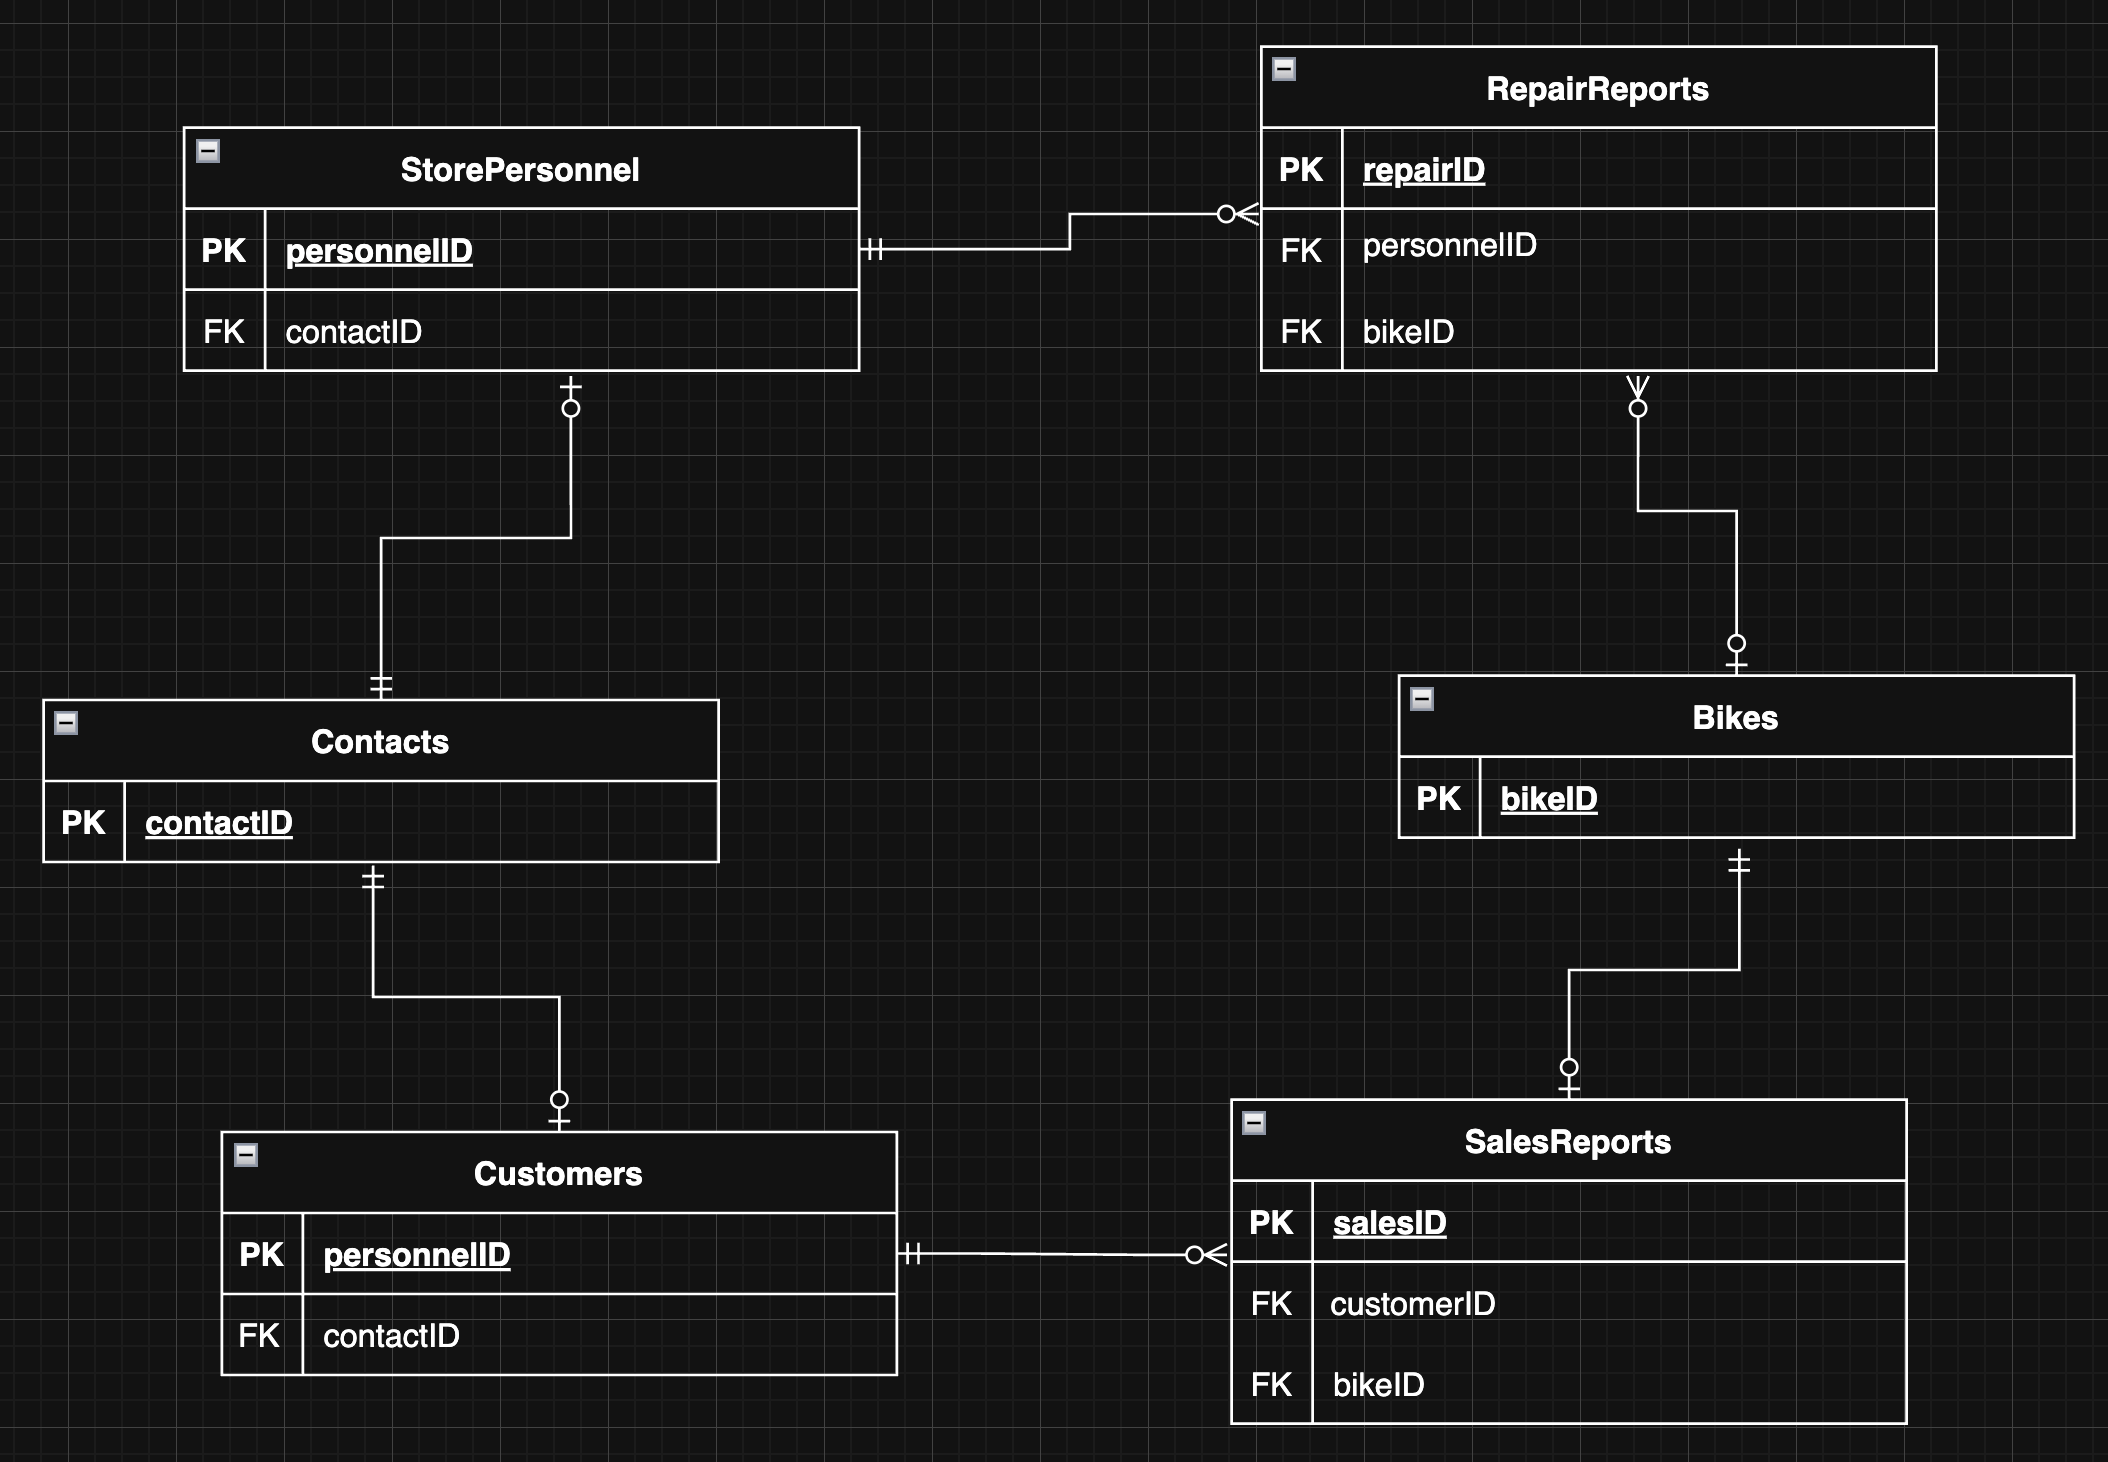
\includegraphics[width=0.9\textwidth]{ERD.png}
\end{center}
\end{tcolorbox}

\vspace{0.5cm}

%%%%%%%%%%%%%%%%%%%%%%%%%%%%%%%%%%%%%%%%%%%%%%%%%%%%%%%%%%%%%
%%%%%%%%%%%%%%%%.                   SECTION 7.                       %%%%%%%%%%%%%%%%%%%%%%%%%
%%%%%%%%%%%%%%%%%%%%%%%%%%%%%%%%%%%%%%%%%%%%%%%%%%%%%%%%%%%%%
\section{Schema Diagram}

\begin{tcolorbox}[colback=secondarycolor, colframe=primarycolor, arc=5mm]

\begin{center}
\vspace{0.5cm}
 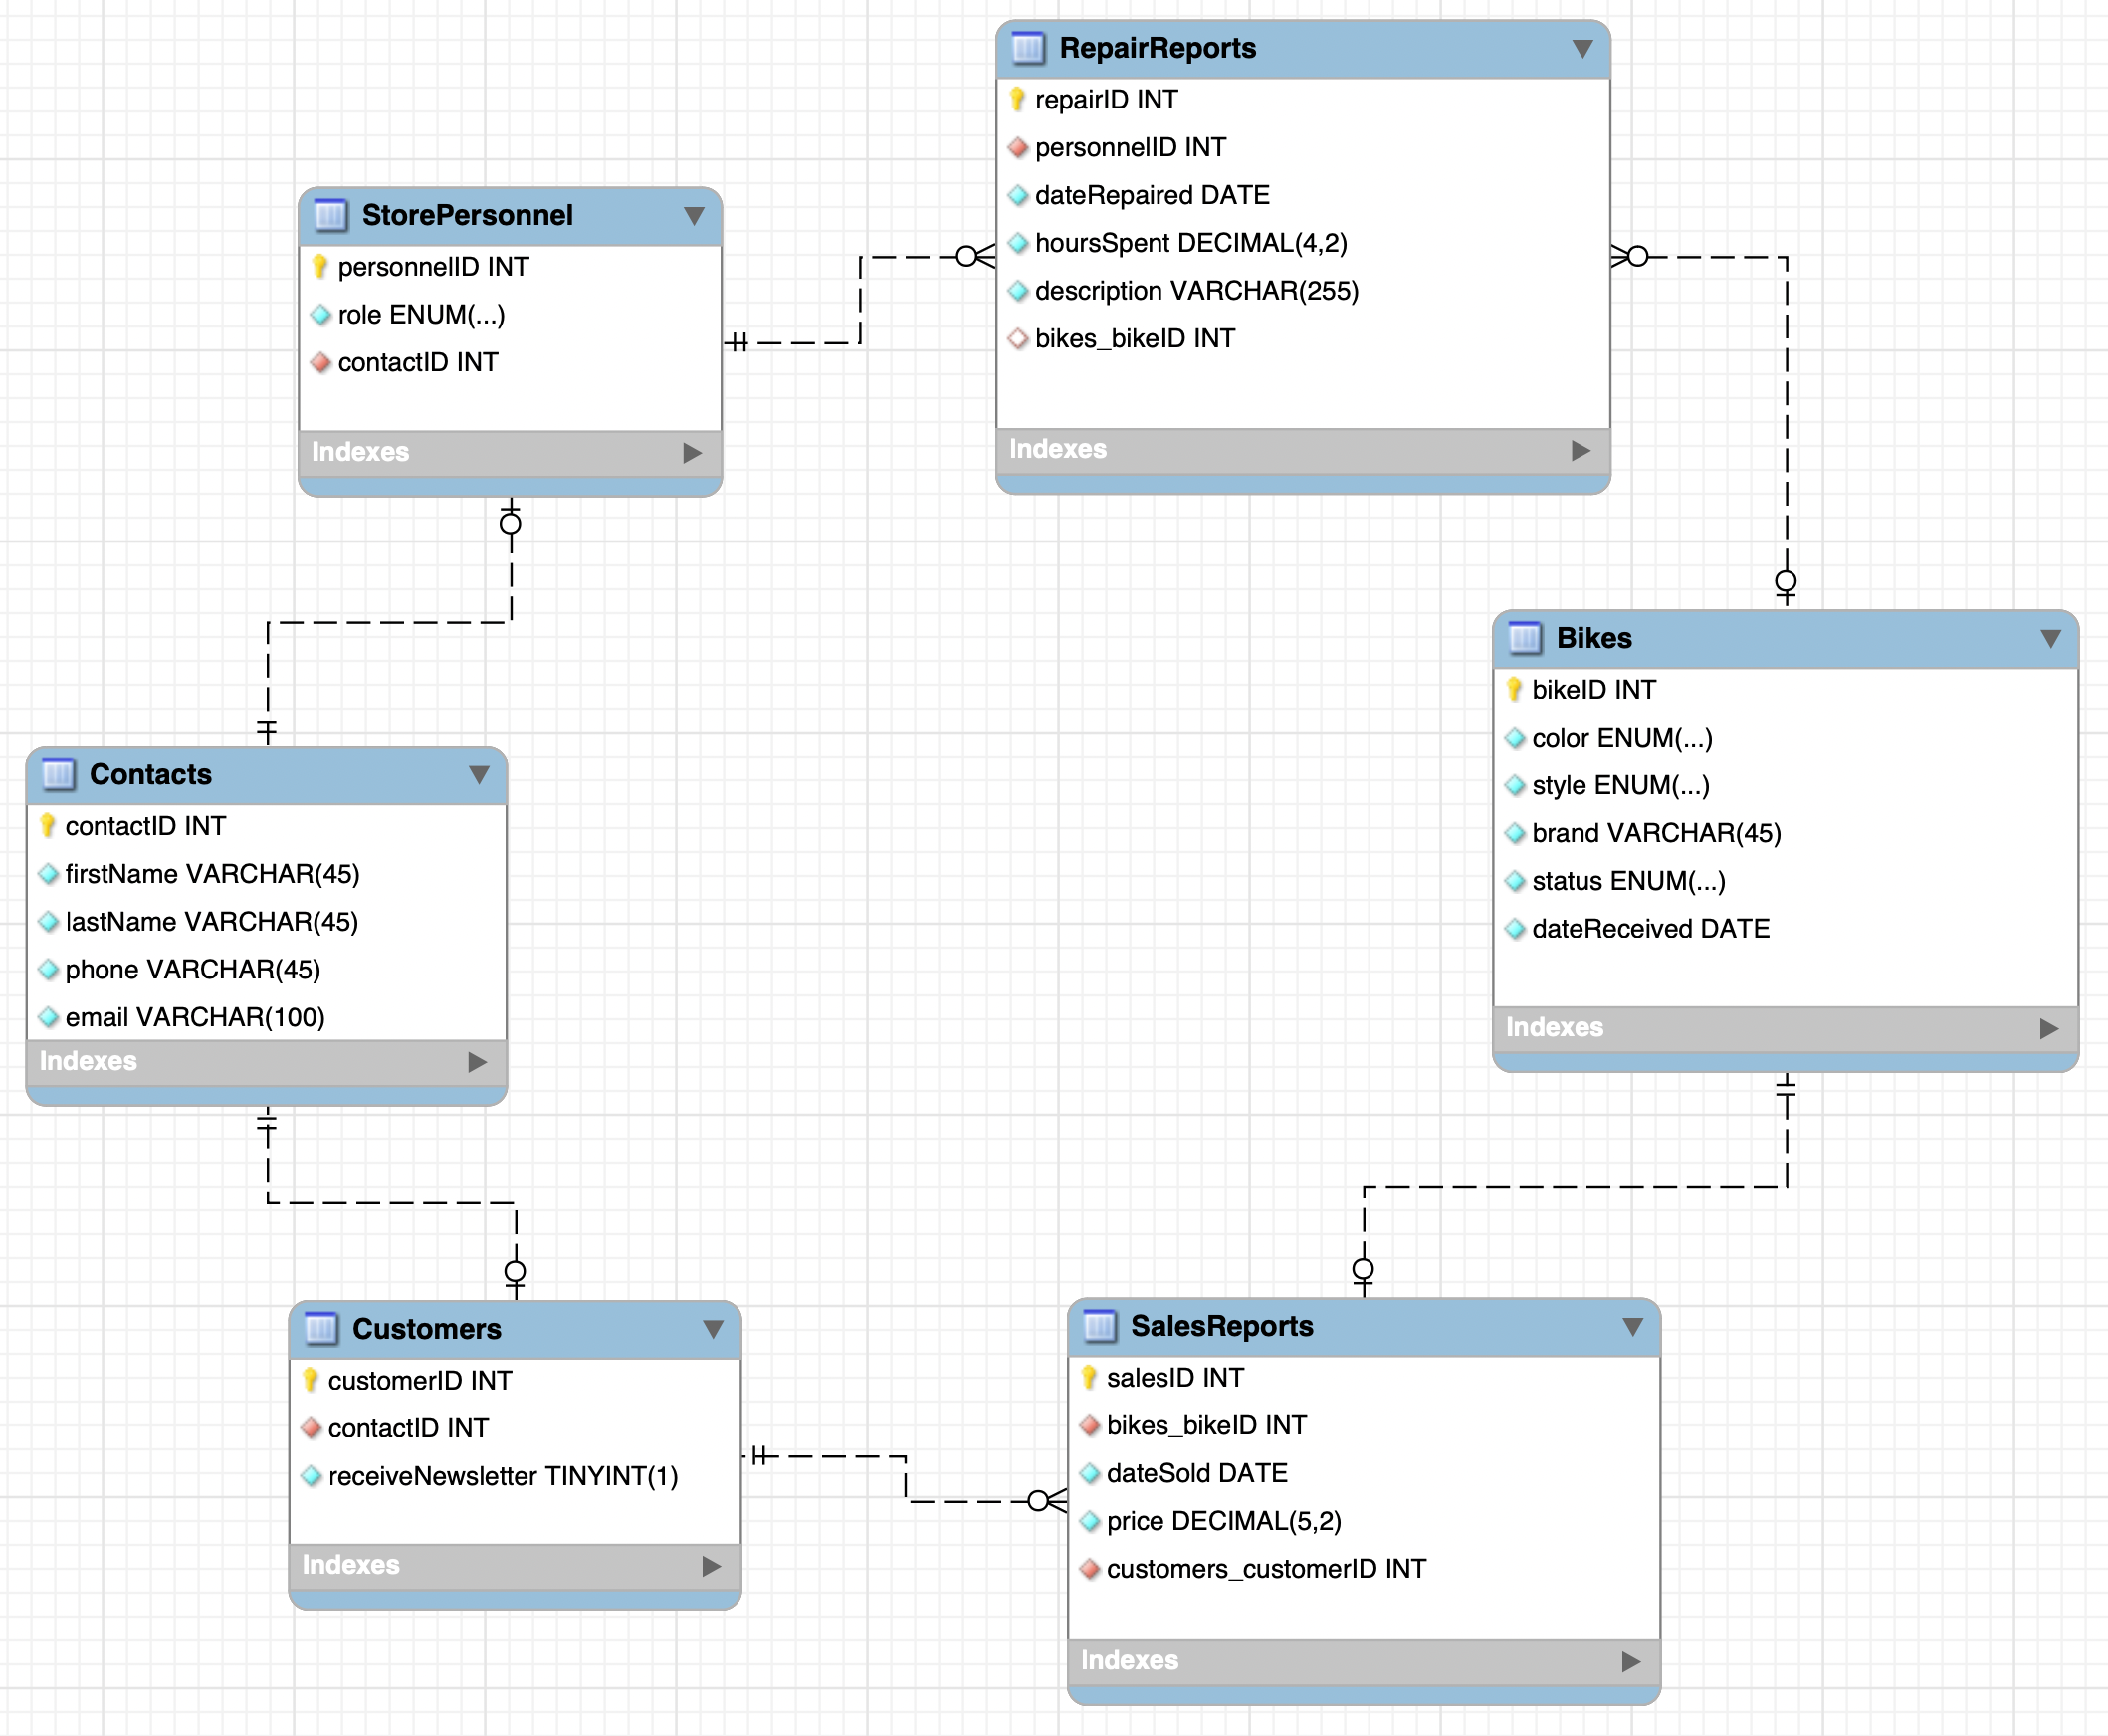
\includegraphics[width=0.9\textwidth]{Schema.png}
\end{center}
\end{tcolorbox}

\vspace{0.5cm}

%%%%%%%%%%%%%%%%%%%%%%%%%%%%%%%%%%%%%%%%%%%%%%%%%%%%%%%%%%%%%
%%%%%%%%%%%%%%%%.                   SECTION 8.                       %%%%%%%%%%%%%%%%%%%%%%%%%
%%%%%%%%%%%%%%%%%%%%%%%%%%%%%%%%%%%%%%%%%%%%%%%%%%%%%%%%%%%%%
\section{Sample Data}

\begin{figure}[H]
    \centering
    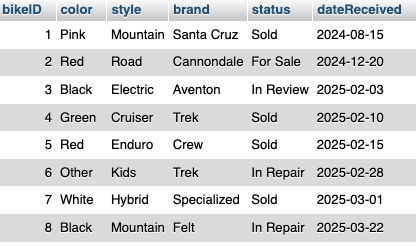
\includegraphics[width=0.5\textwidth]{Bikes.png}
    \caption{Sample data inserted into the Bikes table}
    \label{fig:Bikes}
\end{figure}

\begin{figure}[H]
    \centering
    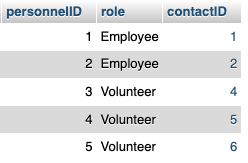
\includegraphics[width=0.5\textwidth]{StorePersonnel.png}
    \caption{Sample data inserted into the StorePersonnel table}
    \label{fig:StorePersonnel}
\end{figure}

\begin{figure}[H]
    \centering
    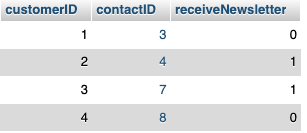
\includegraphics[width=0.5\textwidth]{Customers.png}
    \caption{Sample data inserted into the Customers table}
    \label{fig:Customers}
\end{figure}

\begin{figure}[H]
    \centering
    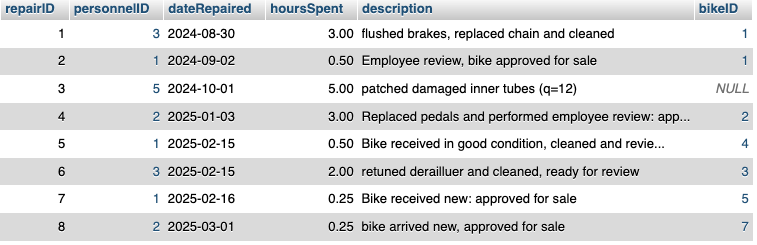
\includegraphics[width=0.5\textwidth]{RepairReports.png}
    \caption{Sample data inserted into the RepairReports table}
    \label{fig:RepairReports}
\end{figure}

\begin{figure}[H]
    \centering
    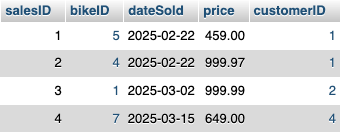
\includegraphics[width=0.5\textwidth]{SalesReports.png}
    \caption{Sample data inserted into the SalesReports table}
    \label{fig:SalesReports}
\end{figure}

\begin{figure}[H]
    \centering
    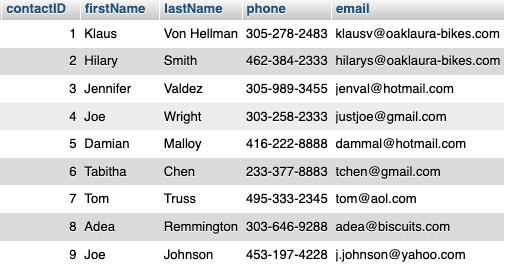
\includegraphics[width=0.5\textwidth]{Contacts.png}
    \caption{Sample data inserted into the Contacts table}
    \label{fig:Contacts}
\end{figure}

%%%%%%%%%%%%%%%%%%%%%%%%%%%%%%%%%%%%%%%%%%%%%%%%%%%%%%%%%%%%%
%%%%%%%%%%%%%%%%.                   SECTION 9.                       %%%%%%%%%%%%%%%%%%%%%%%%%
%%%%%%%%%%%%%%%%%%%%%%%%%%%%%%%%%%%%%%%%%%%%%%%%%%%%%%%%%%%%%
\section{Citations}
\begin{tcolorbox}[colback=secondarycolor, colframe=primarycolor, arc=5mm]
\begin{itemize}
  \item Inspiration for the Bike Co-Op came from The Recyclery, a non-profit bike shop based out of Chicago, IL (last retrieved on 4/9/2025): \href{https://www.therecyclery.org/}{https://www.therecyclery.org/}
  
  \vspace{0.2cm}
  
  \item MySQL workbench was used to create the ERD diagram shown above.
  
  \vspace{0.2cm}
  
  \item The \LaTeX\ template used here was adapted from the Cleese-Assignment template v.2.0 (retrieved on 4/2/2025): \href{https://latextemplates.com/template/cleese-assignment}{https://latextemplates.com/template/cleese-assignment}
  
  \vspace{0.2cm}
  
  \item TeXShop was used for all \LaTeX\ related compilations.
  
  \vspace{0.2cm}
  
  \item All database design work is original.
\end{itemize}
\end{tcolorbox}

\end{document}